\chapter{Applications of Effective SNR}
\label{chap:esnr_eval}

In the previous chapter, we defined the Effective SNR and showed that it can accurately predict packet delivery for 802.11 rates. In this chapter, we explore applications of Effective SNR to various problems of wireless links and wireless networks.

\begin{table}[htp]
	\centering
	\begin{tabular}{lc}
	\toprule
		Application of Effective SNR & Status \\
	\midrule
		Bitrate/MCS selection & \cite{Halperin_ESNR}\\
		Channel width selection & \cite{Halperin_ESNR}\\
		Antenna selection & \cite{Halperin_ESNR}\\
		Power control & \cite{Halperin_ESNR}\\
		Channel selection & \secref{sec:esnr_chansel}\\
		AP selection & \secref{sec:esnr_apsel}\\
		Path selection/BSS selection in WDS & \secref{sec:esnr_pathsel}\\
		Interference planning \\
		Partial packet recovery/FEC & \cite{Bhartia_FreqDiv}\\
		Beamforming \\
		Multicast rate selection \\
	\bottomrule
	\end{tabular}
	\caption{\label{tab:esnr_uses}A variety of applications of Effective SNR\@.}
\end{table}

\tabref{tab:esnr_uses} shows a list of several potential applications of Effective SNR\@. These range from optimizing various parameters of a single Wi-Fi link, such as the MCS or antenna set used, to coordinating many 802.11 nodes in a dense wireless network. Additionally, we identify applications that can be implemented by looking at other aspects of the Channel State Information in \tabref{tab:csi_uses}. These provide useful primitives that can enable systems to adapt behavior based on the location and movement of the user. Combined, we believe these form the critical building blocks for dense 802.11 networks.

\begin{table}[htp]
	\centering
	\begin{tabular}{lc}
	\toprule
		Application of CSI & Status \\
	\midrule
		Mobility classification & \secref{sec:esnr_mobility}\\
		Localization \\
	\bottomrule
	\end{tabular}
	\caption{\label{tab:csi_uses}A variety of applications of Channel State Information.}
\end{table}

In this chapter, we explore CSI and Effective SNR approaches to implementing four of the above applications.

\section{Channel selection}\label{sec:esnr_chansel}


\section{AP selection}\label{sec:esnr_apsel}


\section{Path selection}\label{sec:esnr_pathsel}



\section{Mobility classification}\label{sec:esnr_mobility}
In wireless systems, simply knowing whether a device is mobile can improve performance and reliability. For example, recent work of Ravindranath, et al.\ \cite{Ravindranath_SensorHints} demonstrated a system that improved 802.11a performance on a mobile phone by selecting between different bitrate adaptation algorithms based on whether the device was moving. When the device is static, they use algorithms that can conduct a fine-grained search of the rate space to choose the optimum bitrate. When the device is moving, they use an algorithm that performs a coarser search, but does a better job of tracking a moving optimum. In their experiments, the fine-grained algorithms performed 10--30\% better in static scenarios, while the coarse-grained algorithm performed 25--75\% better in mobile scenarios.

Detecting mobility can also be used to enhance reliability in networks that support dynamic topology, such as today's cellular phone networks, enterprise Wi-Fi wireless distribution systems (WDSes), and networks that support relaying mechanisms such as described above. By proactively looking for a better AP or relay when the device starts moving, service quality can be improved and downtime reduced. \xxx{find some references about cell handoff, WDS handoff, etc.}

The implementation by Ravindranath, et al.\ detected mobility using the accelerometer in a mobile phone. While this technique is accurate and responsive, it has a few disadvantages. The use of an on-board sensor means that detection can only be performed by the mobile client, and thus requires protocol changes to communicate a device's mobile state to the other endpoint of the link, and is not backwards-compatible. Also, this technique can only be implemented on devices that have accelerometers, and requires that this sensor be powered on.

In this section, I explore whether it is possible classify whether a device is mobile based solely on passively measured RF information. If successful, such an implementation would eliminate all of these drawbacks by requiring no extra hardware and supporting unilateral adoption by either endpoint of the link, including the static device. Ravindranath, et al.\ made a preliminary attempt to classify mobility using RSSI, but were not successful. They list several challenges: (1) that RSSI is unstable even for static links in a quiet environment; (2) that RSSI varies by different amounts at different absolute signal strengths, and thus needs to be calibrated; and (3) that RSSI was extremely sensitive to movement in the environment and triggered many false hints. Here, I show that the CSI can overcome these drawbacks and provide a robust solution.

\subsection{Experimental setup}
I configured a SIMO experiment using a single-antenna laptop as the client device, and several of the testbed nodes as three-antenna monitors. The client sent 100,000 back-to-back short packets using MCS0 (1 stream, 6.5\Mbps), approximately one packet every 300\us for 20\s. In my initial data collection described here, I took four traces. Two of the traces were taken with a \emph{static} client in the UW CSE Networking Lab and students present, but not moving in the room. I then took a trace with \emph{environmental mobility} in which I left the client static, but waved my hand within a few centimeters of the antenna and then walked around the room and opened doors. Finally, I took a \emph{mobile device} trace in which I picked up the laptop and moved it around within a meter of its original location. Chronologically, the traces were taken in the order described within a 10-minute window, with the second static trace taken last. \xxx{These results are from only a single receiver and a single mobile experiment; I could look at more traces and conduct more experiments to flesh out the results and to address claim (2) above.}

\subsection{Evaluation}
\topheading{Classifying mobility with RSS\@.} \figref{fig:mobility_rssi} shows the RSS in dBm measured by one receiver for these four traces. Each line shows the RSS for one of the three receive antennas. I note several interesting effects visible in these measurements. First, the RSS is actually extremely stable in static scenarios. This deviation from Ravindranath, et al.\ is likely attributable to the better calibration of the newer 802.11n hardware we use, compared with older hardware used to run experiments with the MadWiFi driver. Second, though RSS does vary with environmental mobility, the variation is fairly small and mostly limited to the periods of activity directly next to the client---later in the trace, when I moved across the room, the RSS variation decreased to the static scenario. It also appears that the variation is not completely correlated across antennas; in several parts of the trace (e.g., at the beginning and around 10--12\s) one or two experience antennas see variation in RSS while the others do not. Finally, the mobile trace exhibits the RSS variation with the largest magnitude, and shows consistent variation throughout the trace and across all antennas. Based on this visual evidence, I conclude it likely that the static scenario can be identified using RSS, and hypothesize that it may also be possible to distinguish between environmental and device mobility. However, I deferred from exploring this possibility further because, as I will show next, the CSI can conclusively classify a device's activity into these three states.

\begin{figure}[htp]
	\centering
	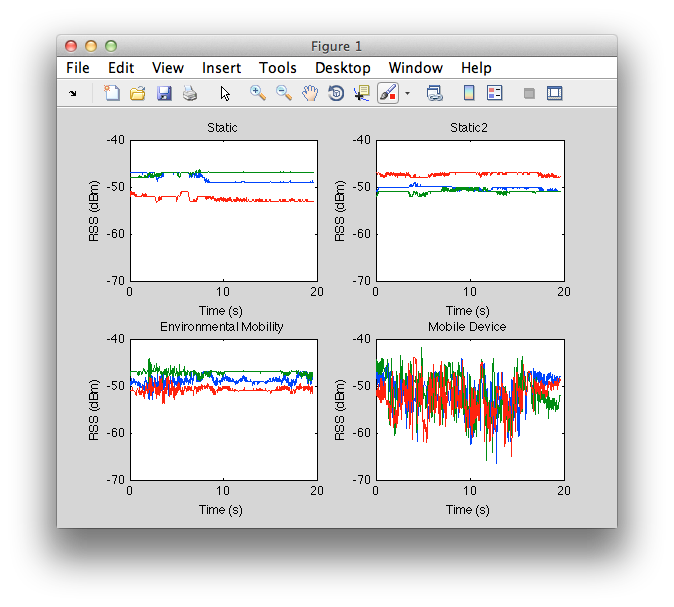
\includegraphics[width=\textwidth]{figures/esnr/mobility_rssi.png}
	\caption{\label{fig:mobility_rssi}RSSI variation in different mobility scenarios.}
\end{figure}

\heading{Classifying mobility with CSI\@.} Here, we examine the same four traces through the lens of the CSI\@. To start, recall that the RSSI yields a single power measurement per sample, whereas the CSI gives a 3-D matrix of complex numbers that represent magnitude and phase on spatial paths and frequency. To quantify the deviation in RSSI, we can simply look at its variation---e.g., absolute difference between samples, or windowed variance---over time. In contrast, we first need a method to quantify the variation in the CSI over time. One simple approach is to use the Pearson correlation function for each spatial path. The Pearson correlation is the ``standard'' correlation function and is defined as
$$
\text{corr}(\vec{x},\vec{y}) = \frac{\sum_{i=1}^n(x_i-\overline{x})(y_i-\overline{y})}{\sqrt{\sum_{i=1}^n(x_i-\overline{x})^2 \sum_{i=1}^n(y_i-\overline{y})^2}}
$$
for $n$-element vectors $\vec{x},\vec{y}$ indexed by $i$ and with respective means $\overline{x}$ and $\overline{y}$. To apply this to CSI, let $\vec{r}_{at}$ represent the magnitudes of the CSI coefficients across subcarriers for antenna $a$ at time sample $t$. Then we can quantify the change between sample $t$ and sample $t+1$ by $\text{corr}(\vec{r}_{at},\vec{r}_{a(t+1)})$.

The correlations for the four traces and for the three received antennas are shown in \figref{fig:mobility_csi}. We see that the static traces show near-perfect correlation, the environmental mobility trace shows a little deviation, and the mobile trace varies wildly with correlations as low as 0.3. \figref{fig:mobility_csi_cdf} shows the CDF of the correlation (combined across antennas) over time. Static traces never show a correlation below 0.98; the trace with environmental mobility never drops to 0.9, and about 3\% of the correlations in the mobile trace are below 0.9. Though the low-correlation outliers occur infrequently, the fact that they are distributed throughout the traces means a windowed thresholding will accurately be able to distinguish between these three states. Note that the mobility state of a device will change slowly---on the order of seconds or longer---and the outliers are frequent enough at this time scale to prevent false negatives.

%In wireless networks today, laptops tend to be ``portable, but not mobile''~\cite{Woodruff_portable}. That is, though they can move from location to location, laptops are infrequently used while actually in motion.

\begin{figure}[htp]
	\centering
	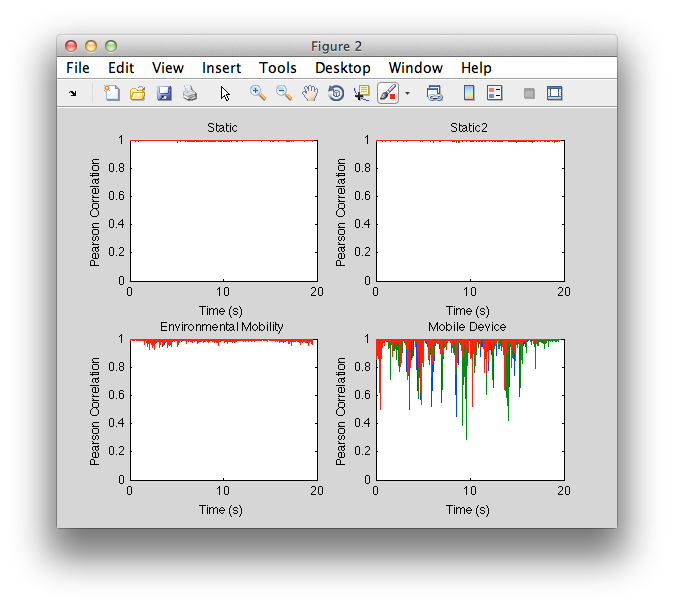
\includegraphics[width=\textwidth]{figures/esnr/mobility_csi.png}
	\caption{\label{fig:mobility_csi}CSI variation as measured by correlation in different mobility scenarios.}
\end{figure}
\begin{figure}[htp]
	\centering
	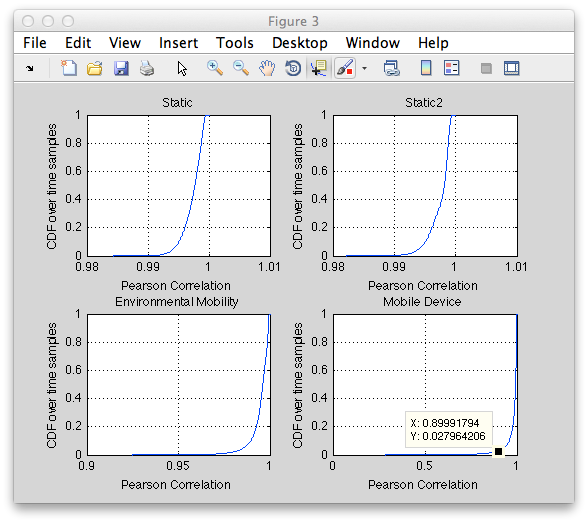
\includegraphics[width=\textwidth]{figures/esnr/mobility_csi_cdf.png}
	\caption{\label{fig:mobility_csi_cdf}CDF of CSI variation as measured by correlation in different mobility scenarios.}
\end{figure}

